\newpage
\section{Diffraction}

\subsection{Single-Slit Diffraction}

We considedr the diffraction parrern of plane waves of light of wavelength $\lambda$ that are diffracted by a single long , narrow slit of width $a$ (aperture) in an otherwise opaque screen $B$. Waves from different points within the slit undergo interference and produce a diffraction pattern of bright and dark fringes on screen $C$. 

\begin{figure}[H]
    \centering
    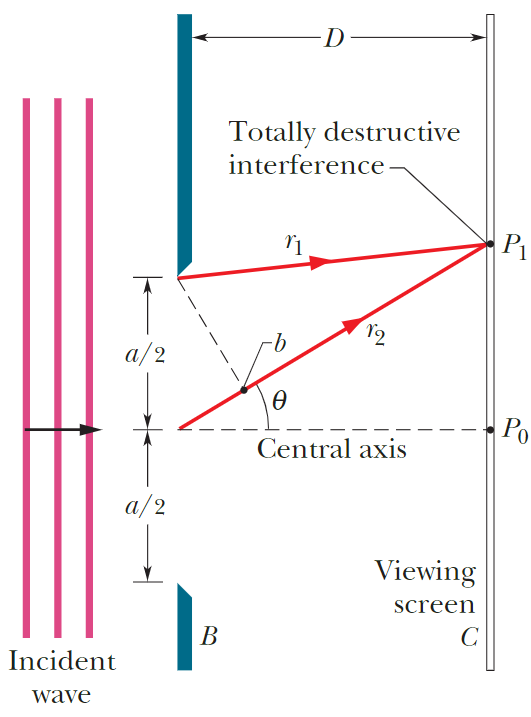
\includegraphics[width=0.209\textwidth]{Lec18/Single-Slit Diffraction}
    \caption{Single-Slit Diffraction}
\end{figure}

\subsubsection{Fraunhofer vs Fresnel Diffraction}
At large screen distance $(D>\frac{a^2}{\lambda})$, the shape of the projected pattern is independent of $D$. This is \highlight{Fraunhofer or far-field diffraction (远场衍射)}. 

At small $D$, however, both the size and shape of the diffraction pattern changes with distance. This phenomenon is known as \highlight{Fresnel or near-field diffraction (近场衍射)}. 

\subsubsection{Locations of the Dark Fringes}
First, we mentally divide the slit into two zones of equal widths $\frac{a}{2}$. We extend $r_1$ and $r_2$ to $P_1$. The wavelets of the pair of rays $r_1$ and $r_2$ are in phase within the slit because they originate from the same wavefront passing through the slit, along the width of the slit. To find the dark fringes, we want the wavelets along these two rays to cancel rech other  when they arrive at $P_1$. So they should be out of phase by $\frac{\lambda }{2}$ when they reach $P_1$. Then any similar pairing of rays from the two zones will give cancellation at the same point $P_1$, because $D\gg a$.Thus we have approximately
\begin{align*}
    \frac{a}{2}\sin\theta=\frac{\lambda}{2}
\end{align*}
The angle $\theta$ of the first dark fringe above and (by symmetry) below the central axis is, therefore, determined by
\begin{align*}
    \sin\theta=\frac{\lambda}{a}
\end{align*}
If we narrow the slit such that $a=\lambda$ , the angle $\theta$ at which the first dark fringes appear increases to $90^{\circ} $. This means that bright fringe must then cover the entire viewing screen. 

\begin{figure}[H]
    \centering
    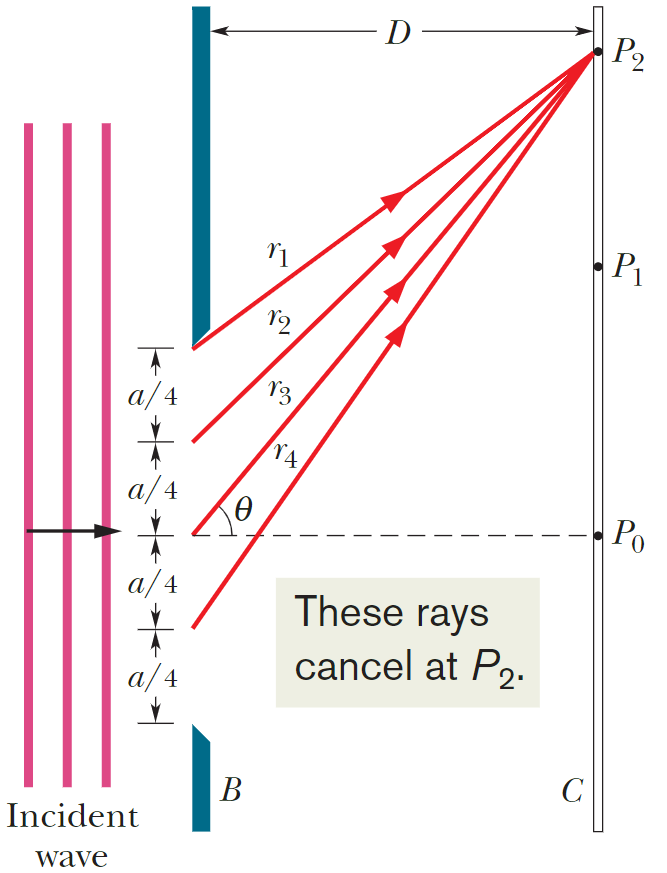
\includegraphics[width=0.209\textwidth]{Lec18/divide the slit into four zones}
    \caption{divide the slit into four zones}
\end{figure}

To find the second dark fringes above and below the central axis, we now divide the slit into four zones of equal width $\frac{a}{4}$. To produce the second dark fringe at $P_2$, the path length difference between $r_1$ and $r_2$, that between $r_2$ and $r_3$, and that between $r_3$ and $r_4$ must all be equal to $\frac{\lambda}{2}$. For $D \gg a$, we can approximately these four rays as being parallel, at angle $\theta$ to the central axis. The path length difference for any two rays that originate at corresponding points in two adjacent zones is $\frac{a}{4}\sin\theta$. Thus we have
\begin{align*}
    \frac{a}{4}\sin\theta=\frac{\lambda}{2}
\end{align*}

We could now continue to locate dark fringes in the diffraction pattern by splitting up the slit into more zones of equal width. We would find that the dark fringes above and below the central axis can be located with the general equation
\begin{align*}
    \frac{a}{2m}\sin\theta=&\frac{\lambda}{2}\\
    a\sin\theta=&m\lambda
\end{align*}
for $m=1,2,3,\dots$. 

In ohter words, in a single-slit diffraction experiment, dark fringes are produced where the path length differences $(a\sin\theta)$ between the top and bottom rays are equal to $\lambda, 2\lambda,3\lambda,\dots$. 

\subsection{Electric Field and Intensity}
To find an expression for the intensity at an arbitrary point $P$ on the viewing screen, corresponding to a particular small angle $\theta$, we need to divide the slit into $N$ zones of equal widths $\Delta x=\frac{a}{N}$ small enough that we can assume each zone acts as a source of Huygens wavelets. We then add the phasors for the wavelets, which form a geometric series (notice $r_{i+1}-r_i=\Delta x\sin\theta$)
\begin{align*}
    \tilde{E}_{\theta}=&\frac{E_0}{N} e^{-i\omega t} \sum_{i=1}^N e^{ikr_i}\\
    =&\frac{E_0}{N}e^{-i\omega t}e^{ikr_1}\times \left[ 1+ e^{ik(r_2-r_1)}+\cdots+e^{ik(r_N-r_1)} \right]
\end{align*}

The arc of phasors represents the wavelets that reach an arbitrary point $P$ on the viewing screen, corresponding to a small angle $\theta$. The amplitude $E_{\theta}$ of the resultant wave at $P$ is the vector sum of these phasors. In the limit of $N \longrightarrow \infty$, the arc of phasors approaches the arc of a circle. 

\begin{figure}[H]
    \centering
    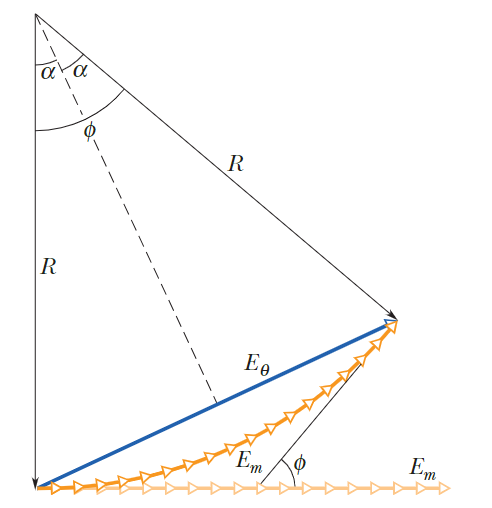
\includegraphics[width=0.209\textwidth]{Lec18/the arc of phasors}
    \caption{the arc of phasors}
\end{figure}

We use a graphic construction
\begin{align*}
    \frac{I(\theta)}{I_{max}}=\frac{E_{\theta}^2}{E_m^2}=\left[ \frac{\left( 2R\sin\alpha \right)^2}{\left( 2R\alpha \right)^2} \right]=\left[ \frac{\sin\alpha}{\alpha} \right]^2
\end{align*}
where $\alpha=\frac{\pi}{\lambda}a\sin\theta$. Noitce $\phi=2\alpha$ is the phase difference bewteen the rays from the top and bottom of the entire slit. 

\begin{figure}[H]
    \centering
    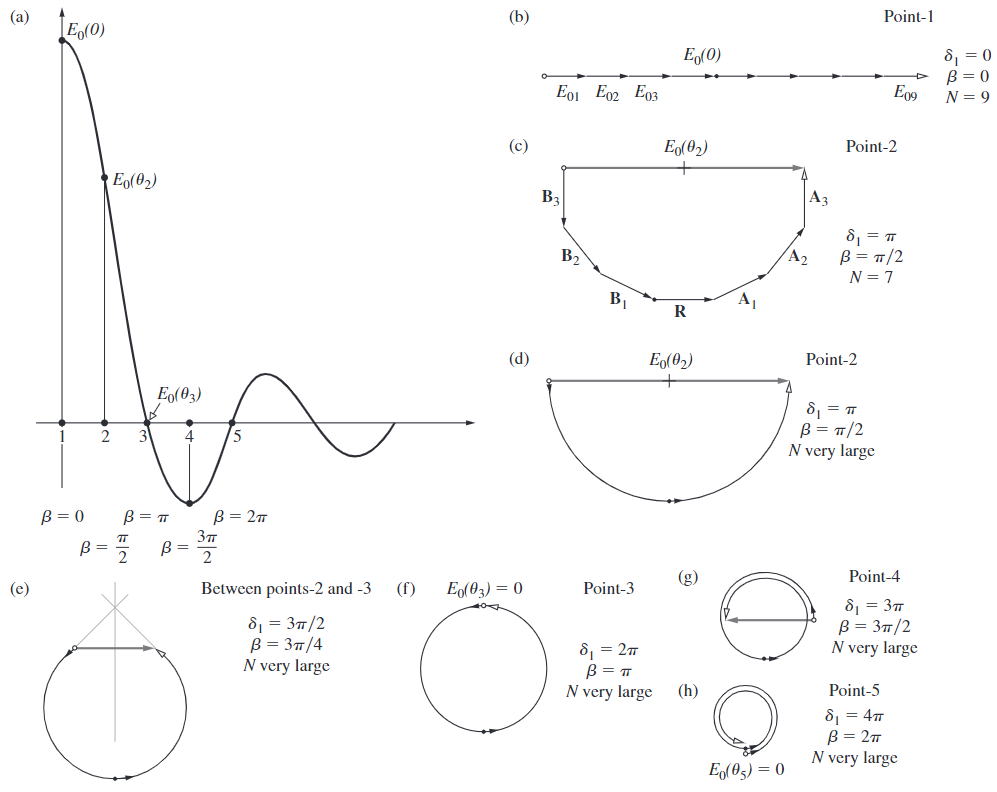
\includegraphics[width=0.489\textwidth]{Lec18/Electric field for single-slit Fraunhofer diffraction}
    \caption{Electric field for single-slit Fraunhofer diffraction. Notice the notation changes $\beta\equiv\alpha$ and $\delta_1\equiv\phi=2\alpha$.}
\end{figure}

As the slit width increases (relative to the wavelength), the width of the central diffraction maximum increases,
the relative height o fthe secondary maxima increases, but the width of the secondary maxima decreases. 

Finally, the geometric serise of phasors is 
\begin{align*}
    \tilde{E}_{\theta}=&\frac{E_0}{N} e^{-i\omega t} \sum_{i=1}^N e^{ikr_i}\\
    =&\frac{E_0 \Delta x}{a} e^{-i\omega t} \sum_{i=1}^N e^{ikr_i}\\
    =&\lim_{N\rightarrow \infty} E_0 e^{-i\omega t}\frac{1}{a}\int_0^a e^{ik(r_1+x\sin\theta)}\,\mathrm{d}x\\
    \sim&\int_0^a e^{ik_x x}\,\mathrm{d} x
    \sim \int_{-\frac{a}{2}}^{\frac{a}{2}} e^{ik_x x}\,\mathrm{d}x
\end{align*}
where $k_x=k\sin\theta$

\begin{figure}[H]
    \centering
    \begin{tikzpicture}[xscale=0.5,yscale=3]
        \draw[<->] (0,1.2)--(0,0)--(12,0);
        \node at (-0.3,-0.1) {$O$};
        \node at (-0.3,1.2) {$f$};
        \node at (12,-0.1) {$\alpha$};

        \draw[light_red, very thick, domain=0.01:3*pi] plot (\x,{pow(sin(\x r)/\x,2)});
        
        \draw[light_green, very thick, domain=0.01:3*pi, samples=100] plot (\x,{pow(sin(\x r),2)});
        \draw[light_green, very thick, domain=0.9:3*pi] plot (\x,{pow(1/\x,2)});

        \node at (pi,-0.1) {$\pi$};
        \node at (2*pi,-0.1) {$2\pi$};
        \node at (3*pi,-0.1) {$3\pi$};
    \end{tikzpicture}
    \caption{$f(\alpha)=\left(\frac{\sin\alpha}{\alpha}\right)^2$, $\sin\theta_{min}=\frac{m\lambda}{a}$}
\end{figure}


\subsection{Fourier Methods in Diffraction Theory}

\subsubsection{Fourier Transform}
The Fourier transform of a one-dimensional function $f(x)$ is defined as 
\begin{align*}
    F(k_x)=\int_{\infty}^{\infty} f(x)e^{-ik_x x}\,\mathrm{d}x
\end{align*}
whose inverse transform is 
\begin{align*}
    f(x)=\frac{1}{2\pi}\int_{\infty}^{\infty}F(k_x)e^{ik_x x}\,\mathrm{d}k_x
\end{align*}

\subsubsection{The Fourier Method for the Single Slit}
Consider the long slit in the y-direction, illuminated by a plane wave. Assuming that there are no phase or amplitude variations across the aperture, the one-dimensional \highlight{aperture function} has the form of a square pulse
\begin{align*}
    E_{sq}(x)=\left\{
        \begin{array}{cc}
            E_0 & |x|\le \frac{a}{2}\\
            0 & |x|>\frac{a}{2}
        \end{array}
    \right.
\end{align*}

The Fourier transform of $E_{sq}(x)$ is
\begin{align*}
    \tilde{E}_{sq}(k_x)=&\frac{1}{a}\int_{-\infty}^{\infty}E_{sq}(x)e^{-ik_x x}\,\mathrm{d}x\\
    =&\frac{E_0}{a}\int_{-\frac{a}{2}}^{\frac{a}{2}} e^{-ik_x x}\,\mathrm{d}x\\
    =&-\frac{E_0}{a}\frac{1}{ik_x}\int_{-\frac{a}{2}}^{\frac{a}{2}} e^{-ik_x x}\,\mathrm{d}-ik_x x\\
    =&-\frac{E_0}{a}\frac{1}{ik_x}e^{-ik_x x}\left|_{-\frac{a}{2}}^{\frac{a}{2}}\right. \\
    =&-\frac{E_0}{a}\frac{1}{ik_x}\left( e^{-ik_x \frac{a}{2}} - e^{ik_x \frac{a}{2}}\right)\\
    \xlongequal{\alpha = \frac{a}{2}k_x}&\frac{E_0}{a} \frac{a}{2}\frac{2i\sin\alpha}{i\alpha}\\
    =&E_0 \frac{\sin\alpha}{\alpha}
\end{align*}
where $\alpha=\frac{a}{2}k_x=\frac{a}{2}k\sin\theta$. 

This leads to the result we have derived
\begin{align*}
    I_{sq}(\theta)=I_{max}\left[ \frac{\sin\alpha}{\alpha} \right]^2
\end{align*}

The key message is that \highlight{the field distribution in the Fraunhofer diffraction pattern is the Fourier transform of the field distribution across the aperture (打到屏幕的光分布是过小孔的光分布的傅里叶变换).}

\begin{figure}[H]
    \centering
    \begin{tikzpicture}[yscale=0.5]
        \draw[xscale=1.5, yscale=0.5, rotate=270, light_red, very thick, domain=-2*pi:0.01] plot (\x,{pow(sin(\x r)/\x,2)});
        \draw[xscale=1.5, yscale=0.5, rotate=270, light_red, very thick, domain=0.01:2*pi] plot (\x,{pow(sin(\x r)/\x,2)});

        \draw [->] (0,-4)--(0,4);
        \draw [->] (-5,-4)--(-5,4);

        \draw [light_red, very thick,|-] (-5,1)--(-5,3);
        \draw [light_red, very thick,|-] (-5,-1)--(-5,-3);
        \draw [light_red, very thick,|-|] (-4,-1)--(-4,1);

        \draw [very thick, ->] (-3.8,0)--(-0.2,0);
        \node at (-2,0.5) {Fourier Transform};
    \end{tikzpicture}
    \caption{The Fourier Method for the Single Slit}
\end{figure}


\subsubsection{The Fourier Method for the Double Silt}

Consider the double slit with its long side in the y -direction, illuminated by a plane wave. Assuming the one-dimensional aperture function along the x direction has the following form
\begin{align*}
    E_{ds}(x)=\left\{\begin{array}{cc}
        0   & |x|<\frac{d-a}{2}\\
        E_0 & \frac{d-a}{2}\le |x| \le \frac{d+a}{2} \\
        0   & |x|>\frac{d+a}{2}
    \end{array}\right.
\end{align*}

The Fourier transform of $E_{ds}(x)$ is 
\begin{align*}
    \tilde{E}_{ds}(k_x)=&\int_{\infty}^{\infty}E_{ds}(x)e^{-ik_x x}\,\mathrm{d}x\\
    =&\int_{-\frac{d+a}{2}}^{-\frac{d-a}{2}} E_0 e^{-ik_x x}\,\mathrm{d} x + \int_{\frac{d-a}{2}}^{\frac{d+a}{2}} E_0 e^{-ik_x x}\,\mathrm{d} x\\
    \xlongequal{x^{\prime}=x+\frac{d}{2}, x^{\prime\prime}=x-\frac{d}{2}}&\int_{-\frac{a}{2}}^{\frac{a}{2}} E_0 e^{-ik_x (-\frac{d}{2}+x^{\prime})}\,\mathrm{d}x^{\prime} \\
    &+ \int_{-\frac{a}{2}}^{\frac{a}{2}} E_0 e^{-ik_x (\frac{d}{2}+x^{\prime\prime})}\,\mathrm{d}x^{\prime\prime}\\
    =&\left( e^{ik_x \frac{d}{2}} + e^{-ik_x \frac{d}{2}}\right)\int_{-\frac{a}{2}}^{\frac{a}{2}} E_0 e^{-ik_x x^{\prime}}\,\mathrm{d} x^{\prime}
\end{align*}
\begin{align*}
    \left( e^{ik_x \frac{d}{2}} + e^{-ik_x \frac{d}{2}}\right) \text{ is double-slit interference}\\
    \int_{-\frac{a}{2}}^{\frac{a}{2}} E_0 e^{-ik_x x^{\prime}}\,\mathrm{d} x^{\prime} \text{ is single-slit diffraction}
\end{align*}

The interference pattern can be understood by a \highlight{convolution theorem} for Fourier transformation: \highlight{The transform of the convolution of two function is the product of their transforms. ($\mathcal{F} [f\circ g]=\mathcal{F}[f]\times \mathcal{F}[g]$)}

The Young's double-slit interference result (with negligible slit width) as the Fourier transform of an aperture function
\begin{align*}
    h(x)=\delta\left(x+\frac{d}{2}\right)+\delta\left(x-\frac{d}{2}\right)
\end{align*}
\begin{align*}
    \mathcal{F}[h(x)]=&\int_{-\infty}^{\infty} h(x)e^{-ikx}\,\mathrm{d}x\\
    =&e^{ik\frac{d}{2}}+e^{-ik\frac{d}{2}}\\
    =&2\cos\left(k\frac{d}{2}\right)
\end{align*}
Notice that 
\begin{align*}
    \delta (x) =&\left\{ \begin{array}{cc}
        1 & x=0\\
        0 & otherwise
    \end{array} \right.\\
    f(a)=&\int_{-\infty}^{\infty}f(x)\delta (x-a)\,\mathrm{d}x
\end{align*}

Therefore, we can express the double-slit aperture function and its Fourier transform as 
\begin{align*}
    E_{ds}(x)=&\int_{-\infty}^{\infty}E_{sq}(x^{\prime})h(x-x^{\prime})\,\mathrm{d}x^{\prime}\\
    \mathcal{F}\left[E_{ds}(x)\right]=&\mathcal{F}\left[E_{sq}(x)\right]\mathcal{F}\left[h(x)\right]
\end{align*}

\begin{figure}[H]
    \centering
    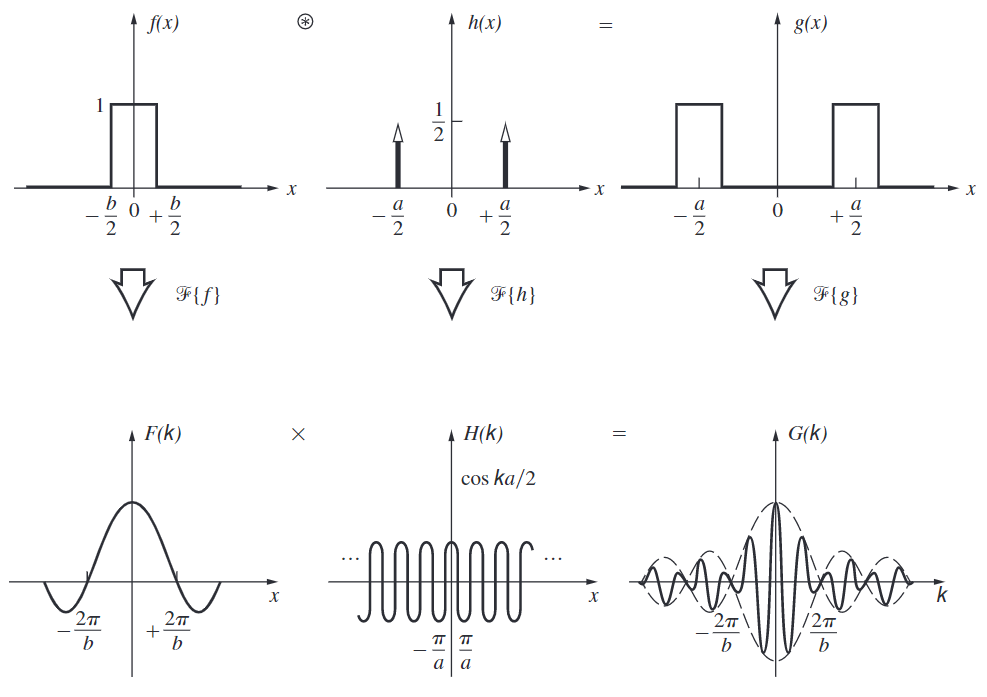
\includegraphics[width=0.48\textwidth]{Lec18/The Fourier Method for the Double Silt}
    \caption{The Fourier Method for the Double Silt}
\end{figure}

Formally, with diffraction effects taken into account, the
intensity of a double-slit interference pattern is

\begin{align*}
    I(\theta)=&I_0\left(\frac{\sin\alpha}{\alpha}\right)^2 \cos^2\beta\\
    \beta=&\frac{\delta_2}{2}=\frac{\pi}{\lambda}d\sin\theta\\
    \alpha=&\frac{\pi}{\lambda}a\sin\theta
\end{align*}

\begin{figure}[H]
    \centering
    \begin{tikzpicture}[xscale=0.8, yscale=3]
        \draw[<->] (0,1.2)--(0,0)--(7,0);
        \node at (-0.3,-0.1) {$O$};
        \node at (-0.3,1.2) {$f$};
        \node at (7,-0.1) {$\alpha$};

        \draw[light_green, very thick, domain=0.01:2*pi] plot (\x,{pow(sin(\x r)/\x,2)});
        \draw[light_green, very thick, domain=0.01:2*pi,samples=100] plot (\x,{pow(cos(2*\x r),2)});
        
        \draw[light_red, very thick, domain=0.01:2*pi, samples=100] plot (\x,{pow(sin(\x r)*cos(2*\x r)/\x,2)});

        \node at (pi,-0.1) {$\pi$};
        \node at (2*pi,-0.1) {$2\pi$};
    \end{tikzpicture}
    \caption{The Fourier Method for the Double Silt}
\end{figure}

The first minimum occurs where the phase difference
between the two slits $(N = 2)$ is 
\begin{align*}
    \delta_2=\frac{2\pi}{\lambda}d\sin\theta=\pi
\end{align*}

The first minimum of the envelope occurs where the phase
difference between one edge and the center of a single slit
is 
\begin{align*}
    \alpha=\frac{2\pi}{\lambda}\sin\theta=\pi
\end{align*}

Therefore, one can determine $\frac{d}{a}$ by counting firnges. In both cases, the larger the length ($d$ or $a$) is, the smaller the $\theta$ ($k_x=k\in\theta$) is. 

\subsection{Diffraction by a Circular Aperture}

Consider diffraction by a circular aperture of diameter d --- that is, a circular opening,  such as acircular lens, through which light can pass. Theimage is nota point, as geometrical optics would suggest,  but a circular disk surrounded by several progressively fainter secondary rings.

\begin{figure}[H]
    \centering
    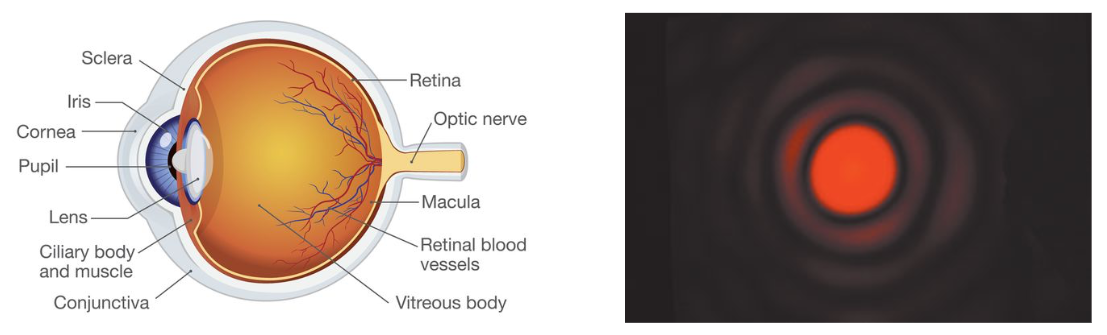
\includegraphics[width=0.309\textwidth]{Lec18/Diffraction by a Circular Aperture}
    \caption{Diffraction by a Circular Aperture}
\end{figure}

We are essentially collecting only a fraction of the incident wavefront and therefore can't hope to form a perfect image. The image is related to the Fourier transform of a disk and is known as the \highlight{Airy pattern}. The analysis of such patterns shows that the first minimum for the diffraction pattern of a circular aperture of diameter $a$ is located by
\begin{align*}
    \sin\theta=1.22\frac{\lambda}{a}
\end{align*}
in contrast to $\sin\theta=\frac{\lambda}{a}$ in the slit case.

The fact that lens images are diffraction patterns is important when we wish to resolve (distinguish) two distant point objects whose angular separation is small. Two objects cannot be distinguished from a single point object, if their diffraction patterns (mainly their central maxima) overlap.

\begin{figure}[H]
    \centering
    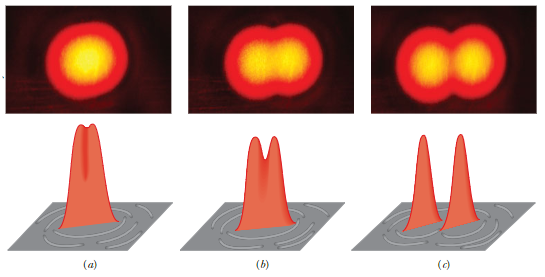
\includegraphics[width=0.309\textwidth]{Lec18/two distant point objects whose angular separation is small}
    \caption{two distant point objects whose angular separation is small}
\end{figure} 

\highlight{Rayleighs criterion} for resolvability states that the two point objects are barely resolved if their angular separation is such that the central maximum of the diffraction pattern of one source is centered on the first minimum of the diffraction pattern of the other, i.e, 
\begin{align*}
    \theta_R=\sin^{-1}\frac{1.22\lambda}{a}\approx 1.22\frac{\lambda}{a}
\end{align*}